\chapter{Solução proposta}
\section{Eletrônica}
\section{Energia}
\section{Estrutura}
\section{Software}

\subsection{Detalhamento dos softwares}
Radares usados no trânsito das cidades necessitam se comunicar com outros sistemas, tanto para passarem as informações obtidas dos automóveis monitorados quanto dados sobre o próprio funcionamento.

Além disso, é necessário às equipes que darão manutenção aos radares terem condições de obterem dados do funcionamento do sistema deles, para decidirem se e qual intervenção necessitarão fazer no equipamento.

Tendo isso em vista, serão 2 as soluções em software para dar suporte ao funcionamento do radar: um serviço -- que fará uso de microsserviços -- para o monitoramento remoto dos radares e uma aplicação a ser usada por equipes de manutenção no diagnóstico dos equipamentos.

Na Figura \ref{fig:diagrama-in-out-software} diagrama que mostra como esses softwares interagirão com o radar:

\begin{figure}[!htb]
    \center{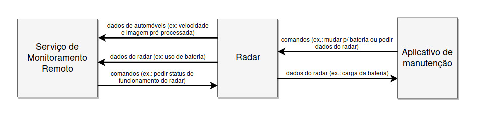
\includegraphics[width=\textwidth]{diagrama-in-out-software}}
    \caption{\label{fig:diagrama-in-out-software} Diagrama de inputs e outputs do radar e dos softwares}
\end{figure}

Nas sessões a seguir, serão melhor detalhados os softwares, assim como as funcionalidades deles.

\subsubsection{Serviço de Monitoramento Remoto (SMR)}
Este serviço, que é um dashboard que possui um servidor de microsserviços que dá suporte a ele, terá a função de obter os dados sobre automóveis enviados pelos radares, receber informações sobre o funcionamento dos equipamentos (por exemplo, se eles estão com a bateria ou os LEDs funcionando) e a partir disso realizar diversas operações.

As funcionalidades desse serviço serão:

\subsubsubsection{Recepção dos dados dos radares}

Os dados enviados por todos os radares serão recebidos pelo SMR e armazenados no banco de dados.

\subsubsubsection{Processamento de imagens de veículos}

As imagens enviadas pelos radares virão pré-processadas. Caberá ao SMR fazer o restante do processamento delas e, a partir disso, pegar as informações da placa dos automóveis.

\subsubsubsection{Verificação da placa do veículo}

O SMR irá checar todas as placas identificadas para saber se o automóvel fotografado foi furtado. Para isso, o SMR acessará o Sinesp ou outro serviço que permita consultar a situação do veículo.

\subsubsubsection{Notificação de irregularidades às autoridades}

Quando um radar fotografar um veículo furtado ou que ultrapassou a velocidade máxima permitida, o serviço irá mandar os dados do automóvel flagrado para as autoridades competentes, para que elas tomem as medidas cabíveis.

Alguns dos dados que serão enviados são a placa, o dia, o horário e a localização do radar que capturou o veículo.

\subsubsubsection{Notificação de possíveis acidentes}

Quando um radar enviar para o serviço uma notificação de possível acidente no local monitorado por ele, o SMR irá notificar uma central que, através de câmeras, irá confirmar se realmente houve um acidente.

Caso não haja câmeras no local, o serviço irá notificar diretamente os bombeiros mais próximos da região onde fica o radar.

\subsubsubsection{Exibição de dados sobre os radares}

O serviço receberá dados sobre todos os equipamentos que se conectarem com ele, como status de funcionamento e problemas com algum componente.

Essas informações poderão ser visualizadas ou usadas em análises de dados.

\subsubsubsection{Exibição de dados enviados pelos radares sobre veículos}

O serviço armazenará os dados sobre as informações relacionadas à veículos enviadas pelos radares, tais como quantidade de imagens enviadas e número de carros flagrados acima da velocidade permitida.

Essas informações poderão ser visualizadas ou usadas em análises de dados.

\subsubsection{Aplicativo de Manutenção}

Esse aplicativo mobile terá como principal objetivo auxiliar as pessoas responsáveis pela manutenção dos radares a diagnosticar como está o funcionamento deles.

As principais funcionalidades dele serão:

\subsubsubsection{Exibição de informações sobre o funcionamento do radar}

Através do aplicativo o responsável pela manutenção poderá saber como está o funcionamento de componentes do radar como, por exemplo, dos LEDs e da bateria.

\subsubsubsection{Alteração da fonte de energia do radar}

Através do aplicativo o responsável pela manutenção poderá mudar a fonte de alimentação do radar para a bateria ou para a fonte de energia externa.

\subsection{Documento de Arquitetura}\label{documento-de-arquitetura}

Esta seção se reserva a informar as decisões tomadas pela equipe de software enquanto a arquitetura de todos os sistemas que forem construídos.

\subsubsection{Finalidade}\label{finalidade}

Esta seção tem como finalidade apresentar uma visão geral arquitetural
do sistemas que compõe a rede de serviços de software para o
\textbf{\emph{RaDop - Radar de Efeito Doppler}}, que será usada como
guia no desenvolvimento do projeto e permitirá um entendimento maior de
todos os componentes integrantes destes sistemas, como um todo, além de
descrever comportamentos, padrões, protocolos de comunicação e demais
informações relacionadas ou correlacionadas. Com o detalhamento da
arquitetura, espera-se, também, deixar explicíta as decisões
arquiteturais realizadas pela equipe.

\subsubsection{Escopo}\label{escopo}

O documento presente abrange três camadas de produtos de software
proposto pela equipe de Projeto Integrador 2 na UnB/FGA, sendo eles um
servidor de serviços/microserviços que darão suporte ao Radar de Efeito
Doppler, com serviços de manipulação de dados, processamento de imagens,
tomada de decisões em tempo real, entre outros. A segunda se trata de um
WebApp de Dashboard, onde estará centralizado grande parte dos dados
providos do Radar com painéis de visualização em tempo real e alguns
dados estatísticos do mesmo. E por fim, o último produto de software se
trata de uma aplicação \emph{mobile} para auxílio de equipes de
manutenção, com dados e informações sobre o equipamento.

\subsubsection{Definições, Acrônimos e Abreviações}\label{definicoes-acronimos-e-abreviacoes}

\begin{itemize}
\tightlist
\item
  \textbf{RaDop}: Nome comercial do Radar produzido pela equipe de
  Projeto Integrador 2.
\item
  \textbf{UnB}: Universidade de Brasília
\item
  \textbf{FGA}: Faculdade Gama
\item
  \textbf{SMR}: Sistema de Monitoramento Remoto
\end{itemize}

\subsection{Produtos de Software}\label{produtos-de-software}

\subsubsection{Servidor de Microserviços RaDop - SMR}\label{servidor-de-microservicos-radop---smr}

A solução de software proposta para o RaDop será composta de um servidor
de serviços/microserviços para realizar tarefas específicas, esses
serviços serão especialistas em tarefas que serão suportadas pelo RaDop,
dessa forma haverá um sistema central que controlará os demais serviços.
A comunicação se dará via API e requisições HTML com transporte, se
necessário, de arquivos JSON com os dados para execução completa e
correta dos serviços. Vale ressaltar que, para sistemas que comunicam
diretamente com componentes eletrônicos do equipamento, o formato de
comunicação pode ser diferente, mas mantendo-se em protocolos de
comunicação em rede, o que pode alterar o formato de transporte de dados
de JSON para um \emph{encoding} mais simples. Os serviços deverão ser
construídos em \href{https://www.python.org/}{python} e/ou em
\href{https://golang.org/}{Go}, podendo ser atribuído a estes uso de
\emph{frameworks}/ferramentas/tecnologias a serem definidas no andamento
do projeto e posteriormente descritos nesta seção. Detalhes da
arquitetura dos mesmos também serão adicionados a posteriori.

\subsubsection{WebApp Dashboard RaDop}\label{webapp-dashboard-radop}

O WebApp Dashboard RaDop será uma aplicação web desenvolvida a partir do
\emph{framework} \href{https://www.djangoproject.com/}{Django}, o qual é
escrito na linguagem de programação
\href{https://www.python.org/}{python}. O \emph{framework} utiliza por
definição o padrão arquitetural \textbf{MVT}, abreviação para
\emph{model}, \emph{view}, \emph{template}, que é derivada do padrão
arquitetural \textbf{MVC}, \emph{model}, \emph{view}, \emph{controller},
amplamente utilizada para esta finalidade e largamente aceita pela
comunidade produtora de software. De acordo com o \emph{site}
DjangoBook, a parte de \emph{controller}, em Django, é tratada pelo
próprio \emph{framework}. Portanto a \emph{View} do \textbf{MVT}
desempenha um papel próximo, mas não igual ao \emph{controller}.

As camadas desse tipo de arquitetura estão descritas no seguinte
formato, abaixo.

\subsubsubsection{\emph{Model}}\label{model}

É uma representação do banco de dados. Além disso, também inclui
características, relações e outros comportamentos que os dados podem
assumir.

O Django inclui varias ferramentas para automatizar tanto quanto
possível o processo e a manipulação do banco de dados, de forma que o
desenvolvedor não precise se preocupar tanto com o banco de dados, o que
ajuda no foco do desenvolvimento da aplicação de forma mais rápida.

\subsubsubsection{\emph{View}}\label{view}

Estabelece uma ponte entre a \emph{Models} e o \emph{Templates}. Recebe
as requisições do usuário a partir do \emph{template}, acessa o banco de
dados e então retorna a informação solicitada pelo usuário, por meio de
HTML, XML e/ou os erros encontrados.

\subsubsubsection{\emph{Template}}\label{template}

Agrega toda a parte visual que estará visível para os usuários. Inclui
os códigos HTML, CSS, JavaScript, entre outras linguagens que são
utilizadas na apresentação da \emph{View}/\emph{Front-end} ao usuário.

\subsubsection{Aplicativo RaDop}\label{aplicativo-radop}

O aplicativo RaDop será uma aplicação mobile desenvolvida a partir do
\emph{framework} \href{https://facebook.github.io/react-native/}{React-Native}, construído em cima da
linguagem de programação \href{https://www.javascript.com/}{JavaScript}. O
React-Native é o que chamamos de \emph{data-driven}, ou seja, ele não
implementa padrões arquiteturais por padrão, apenas utiliza os dados que
recebe (basicamente as funções recebem os dados e devolvem resultados).
No caso do React os dados são o estado da aplicação, as controllers são
as funções são os componentes e os resultados são a UI. Dessa forma, a
aplicação é modularizada em \textbf{N} componentes, como dito por Jensen \cite{jensen2018} (podendo ser
\emph{stateless} ou \emph{stateful}), o que torna a aplicação escalável,
robusta e de fácil manutenção.

\subsubsubsection{\emph{Stateless}}\label{stateless}

Neste formato de componente apenas recebe dados de outros componentes
para a sua execução, isso infere que cada uma de suas execuções é
independente, portanto não há conexão entre uma transação e outra. Com
isso o componente não retém dados para si, ou estado de sessões,
propriedades, execuções ou outras informações quaisquer em sua
estrutura.

\subsubsubsection{\emph{Statefull}}\label{statefull}

Neste formato o componente controla o seu próprio estado, ou seja, ele
armazena informações de sua própria execução e subsequentemente, como o
próprio nome diz, do seu estado. Com isso, também, o componente fica
responsável pelo envio dessas informações para outros componentes.

\subsection{Requisitos e Restrições Arquiteturais}\label{requisitos-e-restricoes-arquiteturais}

\subsubsection{Servidor de Microserviços RaDop - SMR}\label{req-servidor-de-microservicos-radop---smr}

\begin{table}[h]
  \resizebox{\textwidth}{!}{\begin{tabular}{|r|l|}
  \hline
  \textbf{Requisito} & \textbf{Ferramenta/Solução}                                                                                                                                                                                                                                                           \\ \hline
  Linguagem & Python 3.7.3 e Go 1.12                                                                                                                                                                                                                                                                         \\ \hline
  Framework & WebSocket, API Rest e Outros                                                                                                                                                                                                                                                                   \\ \hline
  Segurança & \begin{tabular}[c]{@{}l@{}}Os dados utiizados nos serviços/microsserviços\\ de apoio serão armazenados apenas para\\ auditórias e uso em estatísticas/mining/BI,\\ sendo possível o agendamento da remoção\\  dos mesmos para manter sigilo de dados pessoais,\\ caso necessário.\end{tabular} \\ \hline
  \end{tabular}}
  \caption{Restrições e Requisitos para a construção dos microsserviços propostos.}
\end{table}

\subsubsection{WebApp Dashboard RaDop}\label{req-webapp-dashboard-radop}

\begin{table}[h]
  \resizebox{\textwidth}{!}{\begin{tabular}{|r|l|}
  \hline
  \textbf{Requisito}  & \textbf{Ferramenta/Solução}                                                                                                                                                                                                                                       \\ \hline
  Linguagem  & Python 3.7.3                                                                                                                                                                                                                                                               \\ \hline
  Framework  & Django 2.1.7                                                                                                                                                                                                                                                               \\ \hline
  Plataforma & Web - Navegadores Google Chrome, Apple Safari e Mozilla Firefox                                                                                                                                                                                                            \\ \hline
  Segurança  & \begin{tabular}[c]{@{}l@{}}Todas as informações dos usuários da dashboard\\ devem ser tratadas em sigilo para que\\ apenas o próprio usuário possa visualizá-las,\\  demais informações não serão\\ armazenadas a fim de manter sigilo de dados\\ dos mesmos.\end{tabular} \\ \hline
  \end{tabular}}
  \caption{Restrições e Requisitos para construção do sistema em Django.}
\end{table}

\subsubsection{Aplicativo RaDop}\label{req-aplicativo-radop}

\begin{table}[h]
\centering
  \begin{tabular}{|r|l|}
  \hline
  \textbf{Requisito} & \textbf{Ferramenta/Solução}  \\ \hline
  Linguagem          & JavaScript ES 6              \\ \hline
  Framework          & React-Native 0.59            \\ \hline
  Dependências       & Java Oracle JDK 8 e Node 11+ \\ \hline
  Plataforma         & Mobile - Android 4+          \\ \hline
  \end{tabular}
  \caption{Restrições e Requisitos para construção do sistema em React-Native.}
\end{table}

\subsection{Visão Lógica}\label{visao-logica}

\subsubsection{Serviços RaDop}\label{servicos-radop}

A visão lógica dos serviços do RaDop serão melhor apresentados durante a
execução do projeto devido ao fato da necessidade de cada serviço ser
única não permitir apenas uma representação lógica dos mesmos.

\subsubsection{WebApp Dashboard RaDop}\label{visao-webapp-dashboard-radop}

A visão lógica do WebApp Dashboard está descrita na Figura 2.

\begin{figure}[!htb]
    \center{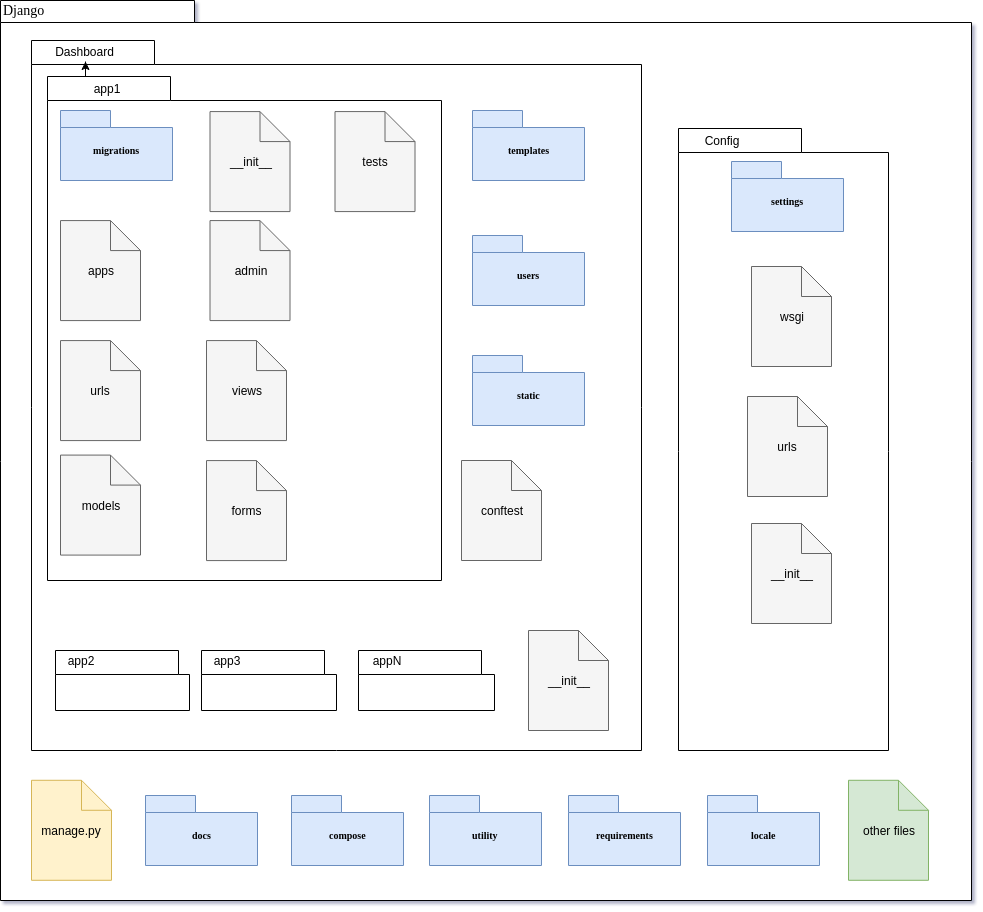
\includegraphics[width=\textwidth]{diagrama-pacotes-django}}
    \caption{\label{fig:diagrama-pact-django} Diagrama de Pacotes Django}
\end{figure}

\subsubsection{Aplicativo RaDop}\label{visao-aplicativo-radop}

A visão lógica do Aplicativo está descrita na Figura 3.

\begin{figure}[!htb]
    \center{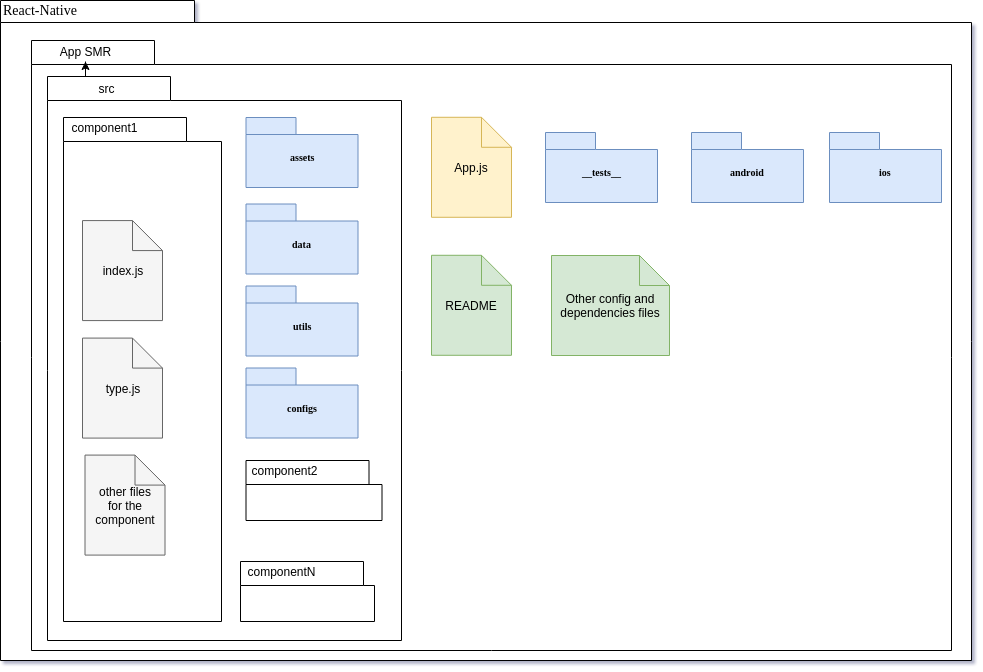
\includegraphics[width=\textwidth]{diagrama-pacotes-react}}
    \caption{\label{fig:diagrama-pact-react}Diagrama de Pacotes React}
\end{figure}

\subsection{Tamanho e Desempenho}\label{tamanho-e-desempenho}

Devido a necessidade de decisões em tempo real os sistemas críticos
deverão ser desenvolvidos de modo a serem o mais perfomáticos possível,
num ponto de vista de tempo de execução, tempo de recebimento de dado e
tempo de envio de dados (excluíndo de fatores externos), e que sejam
capaz de se recuperar de falhas, sejam de redes, de execução e etc. Os
demais sistemas que não forem críticos deverão seguir os melhores
padrões da comunidade produtora de software, afim de manter o seu
tamanho e desempenho dentro de parâmetros aceitáveis pelos
\emph{stakeholders} do projeto.

\subsection{Qualidade}\label{qualidade}

A qualidade das três camadas de produto software para o Radar de Efeito
Doppler - RaDop se darão pelos padrões definidos na comunidade, sendo
avaliado legibilidade de código dado pelo padrão de estilo de escrita,
como o \href{https://www.python.org/dev/peps/pep-0008/}{PEP 8} definido
pelo python, cobertura de código via testes unitários e presença de
testes unitários para funções dos módulos dos sistemas/serviços. As
interfaces visuais serão testadas para serem usáveis, interativas e de
fácil aprendizado, sendo essas validadas com os \emph{stakeholders} do
projeto e com os integrantes da equipe.
